% --- Guidance and sampling ---
\section{Guidance and Sampling}
\begin{frame}[plain]
    \centering
    \vspace{2cm}
    {\Huge \textcolor{blue}{Stable Diffusion:}\\[1em]
     \textbf{Guidance and Sampling}}
\end{frame}

\begin{frame}{Classifier-Free Guidance (CFG)}
  \begin{itemize}\itemsep0.3em
    \item Conditioning alone follows the prompt only loosely; every real system amplifies it with \textbf{classifier-free guidance} (Ho \& Salimans, 2022).
    \item \textbf{Training trick:} randomly drop the text conditioning for a fraction of training steps ($\sim$10\%), so one network learns both a \textbf{conditional} and an \textbf{unconditional} noise prediction.
    \item \textbf{At sampling time}, run both and \textbf{extrapolate}:
    \[
    \hat{\epsilon} = \epsilon_\theta(x_t, \varnothing) + w \left[ \epsilon_\theta(x_t, c) - \epsilon_\theta(x_t, \varnothing) \right]
    \]
    \item The guidance scale $w$ trades \textbf{prompt fidelity} against \textbf{diversity}: $w = 1$ is plain conditional sampling; SD v1 defaults to $w \approx 7.5$; too high causes oversaturated, artifact-prone images.
  \end{itemize}
\end{frame}

\begin{frame}{CFG, Geometrically}
  \begin{figure}
    \centering
    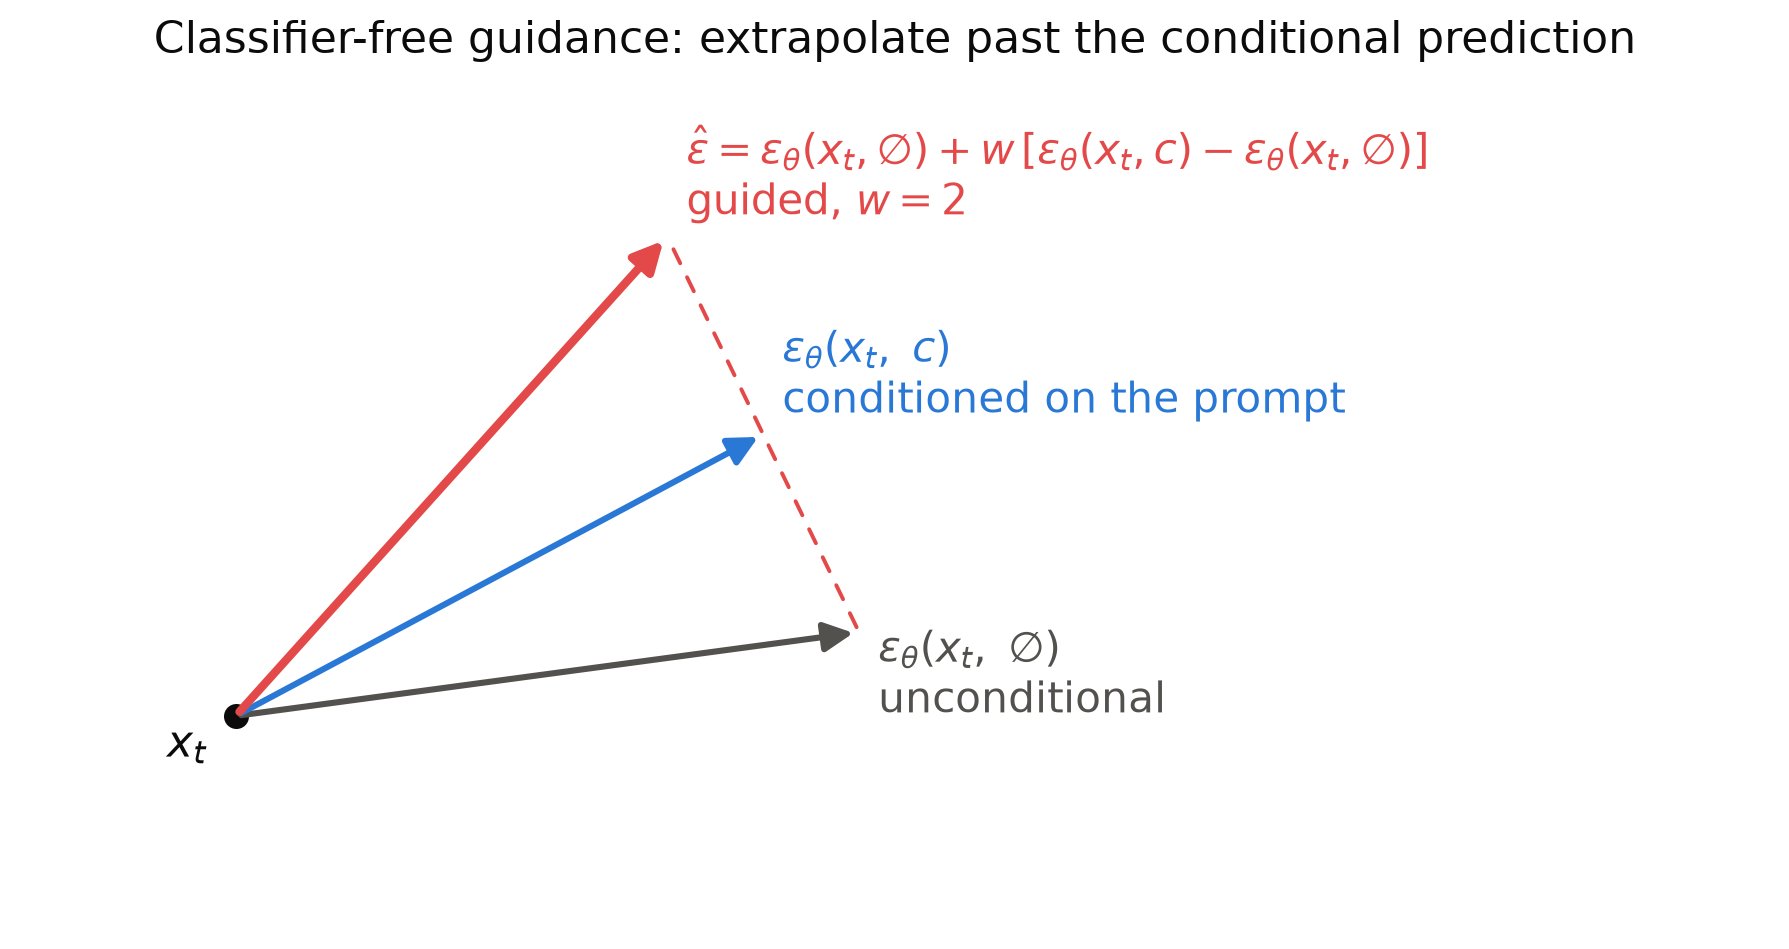
\includegraphics[height=0.5\textheight, width=\textwidth, keepaspectratio]{images/stable-diffusion/cfg_guidance_vectors.png}
  \end{figure}
  \begin{itemize}
    \item Each denoising step pushes the sample \textbf{past} the conditional prediction, away from the unconditional one: whatever the prompt adds gets amplified.
    \item \textbf{Negative prompts} reuse the same mechanism: replace the unconditional branch with an embedding of what you do \emph{not} want, and the extrapolation pushes away from it.
  \end{itemize}
\end{frame}

\begin{frame}{Samplers: From 1000 Steps to 20}
  \begin{itemize}\itemsep0.28em
    \item DDPM training uses $\sim$1000 noise levels, but sampling does not have to visit all of them.
    \item \textbf{DDIM} (Song et al., 2021): a deterministic sampler over the same trained model; skips steps and enables consistent latent-space edits. Typically 20--50 steps.
    \item \textbf{ODE-solver view:} sampling is integrating a differential equation, so higher-order solvers (DPM-Solver++, Euler variants in practice) reach good quality in fewer steps.
    \item \textbf{Distillation} goes further, to 1--4 steps: latent consistency models (LCM), adversarial diffusion distillation (SDXL Turbo), and SD 3.5 \textbf{Large Turbo} all distill a many-step teacher into a few-step student.
    \item Practical takeaway: the model, the sampler, and the step count are \textbf{independent choices}; most quality-speed tuning happens here.
  \end{itemize}
\end{frame}
